\chapter[Clustering Uncertain Data Based on GLD Similarity]{Clustering Uncertain Data Based on GLD Similarity}\label{cap:gld_clustering}

In Chapter \ref{cap:gld} we exposed the two most important parameterizations of the \textit{GLD} and select the \textit{FMKL} as  the one to be used for the rest of the  thesis. In this parameterization $\lambda_{1}$ represent the location of the \textit{GLD} and is directly related to the mean of the distribution. $\lambda_{2}$ is the scale, directly related to the standard deviation; and $\lambda_{3}$ and $\lambda_{4}$ represent the left and right tails of the distribution. Combinations of $\lambda_{3}$ and $\lambda_{4}$ can be used to estimate the skewness and kurtosis of the distribution.

As $\lambda_{2}$ define the dispersion, and $\lambda_{3}$ and $\lambda_{4}$ the shape of a \textit{GLD}, so the combination of those parameters are the responsible of the quantification of the uncertainty, from the \textit{GLD} point of view.

The \textbf{RQ.1} we formulate in the Introduction (see Chapter \ref{cap:intro}) is:

\begin{tcolorbox}
\textbf{RQ1.} how to group the output of the UQ process based on the similarity of the uncertainty?
\end{tcolorbox}

If the uncertainty in a \textit{GLD} is characterized by $\lambda_{2}$, $\lambda_{3}$ and $\lambda_{4}$ and we are interesting into group the uncertainty based on the similarity, is clear that we need to explore how to group the \textit{GLDs} based on its $\lambda$ values. This is the main objective of this Chapter, that is organized as follow: in Section \ref{sec:related_works} a brief review of some related works is performed, and the advantage and drawbacks of those works are highlighted. Some considerations about the possibilities of the use of the \textit{GLD} to solve some of the drawbacks are commented. Next, in section \ref{sec:clustering_gld} our hypothesis about the use of the \textit{GLD} to clustering uncertain data, is presented. Sections \ref{sec:synthetic_I} and \ref{sec:synthetic_II} present two synthetics datasets and the results of the clustering technique. Those results help us to validate our hypothesis. Finally, section \ref{sec:clustering_summary} summarize and discuss the main results of the Chapter.

\section{Related Works}\label{sec:related_works}
Clustering uncertain data is recognized as an essential tasks in mining uncertain data \cite{Jiang2011}. It impose significant challenges in both modeling similarities between uncertain objects and developing efficient computational methods. Many methods are implemented as extensions of k-means and density-based clustering methods like DBSCAN, but using geometric distances between objects. Such methods cannot handle uncertain objects that are geometrically indistinguishable, such as products with the same mean but very different variances, as the uniform and normal distributions in Figure \ref{fig:normal_uniform}.

\begin{figure}[H]
    \centering
    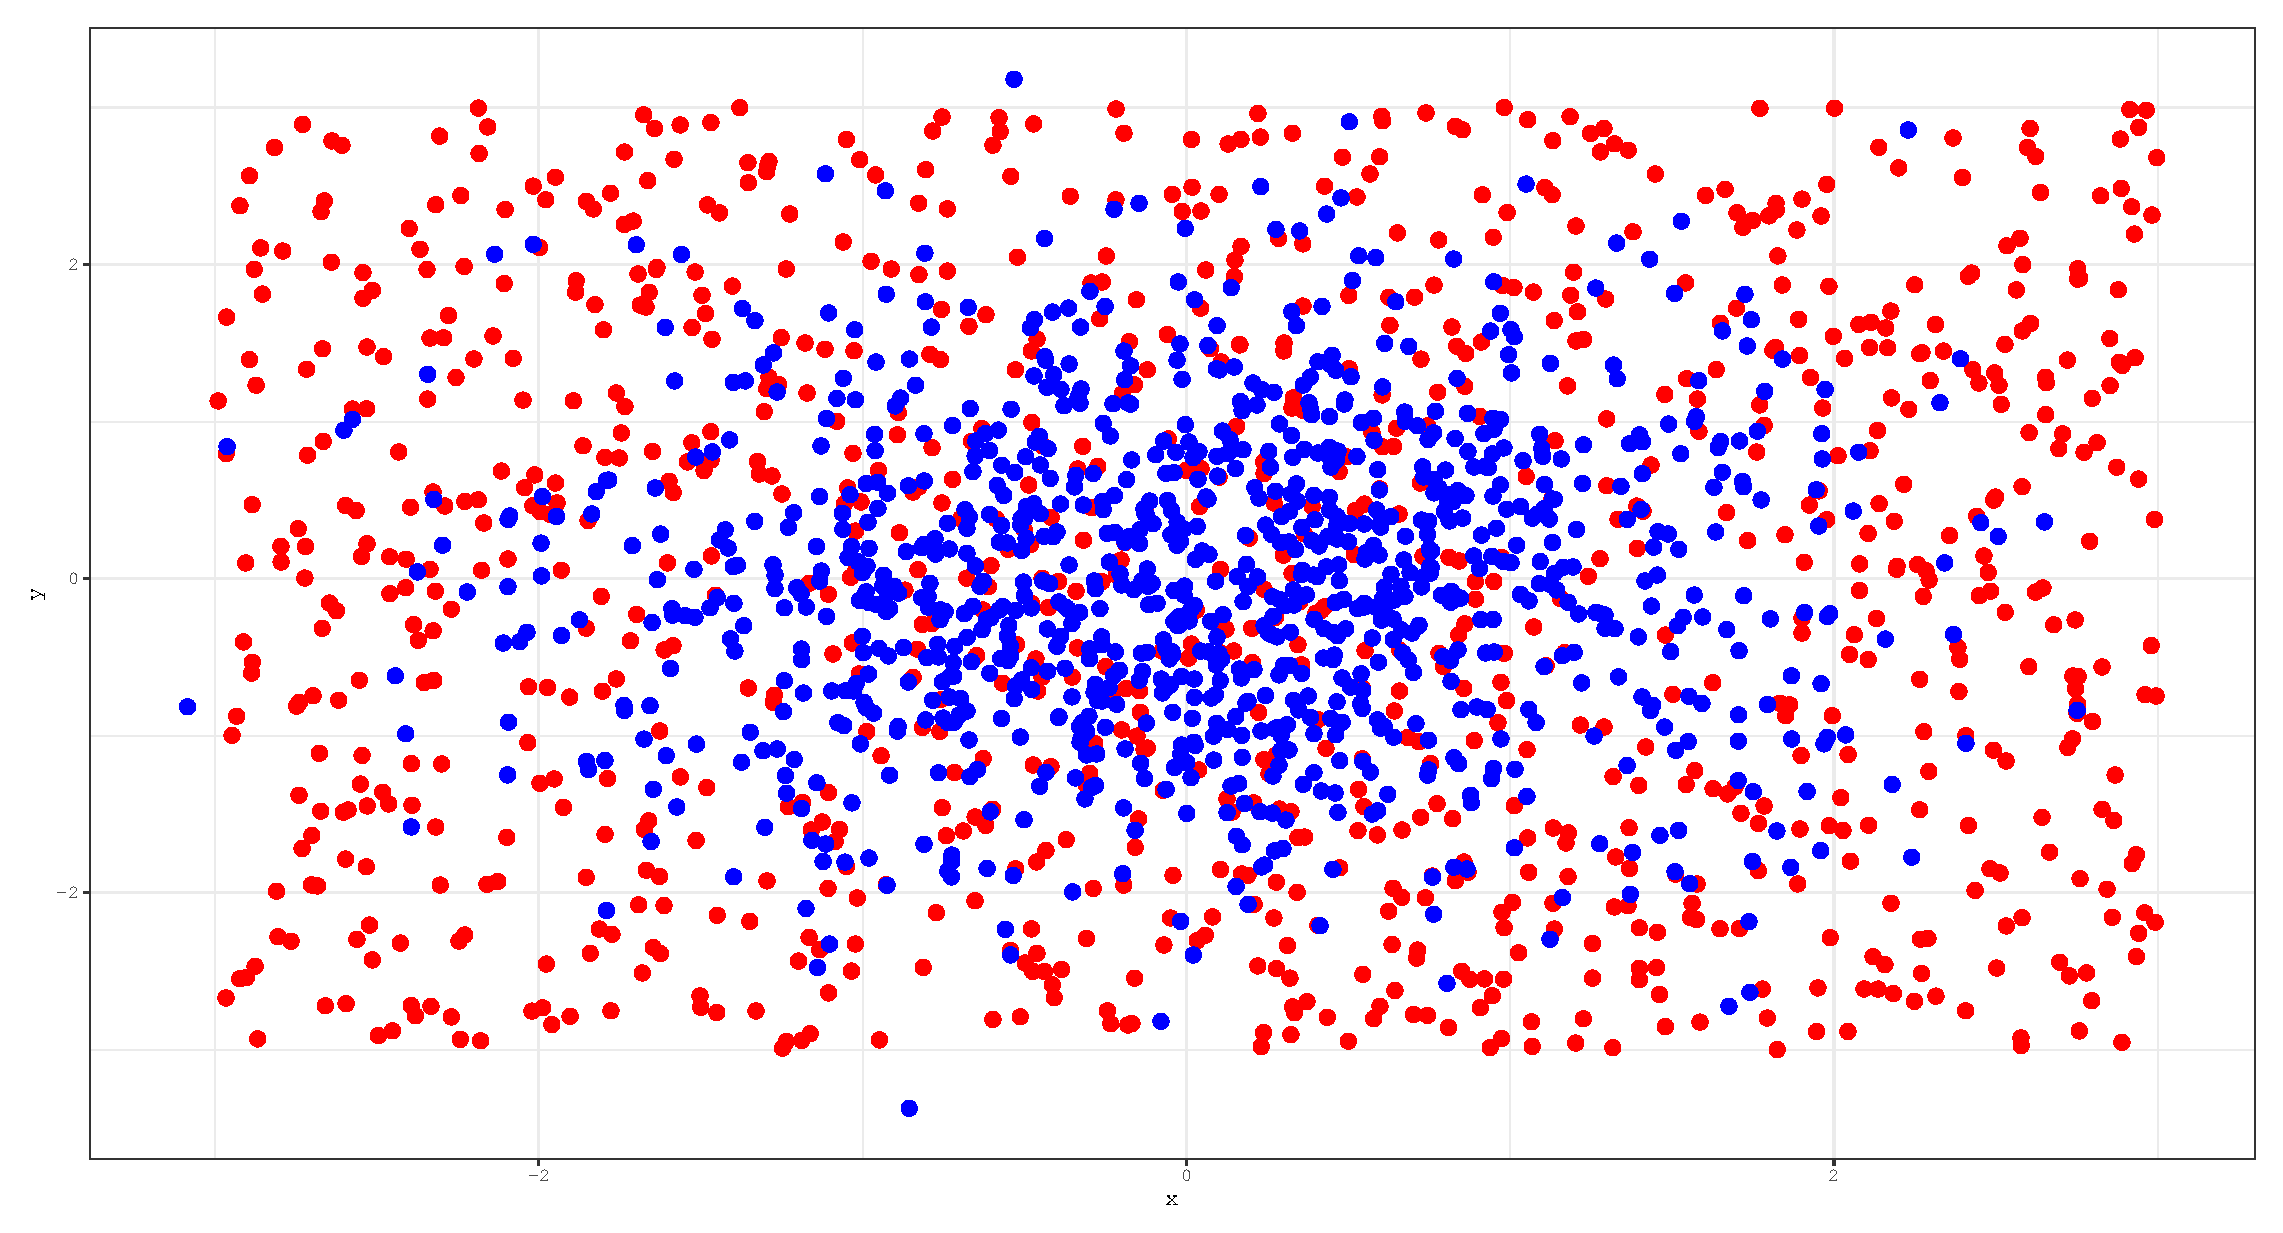
\includegraphics[width=0.8\textwidth]{img/gld_clustering/normal_uniform.eps}
    \caption{Two geometrically indistinguishable distributions. Both distributions have the same mean but different variances. In color blue a bivariate Gaussian distribution, in red a bivariate uniform distribution.}
    \label{fig:normal_uniform}
\end{figure}

Until recently, probability distributions, which are essential characteristics of uncertain objects, had not been considered in measuring the similarity between uncertain objects. In the last years, a plethora of new methods to clustering uncertain data emerge, based in the use of statistical metrics like Kullback-Leibler divergence (KL-divergence). From the best of our knowledge, the first effort in this direction was the work of Jiang et al. \cite{Jiang2011}, where they propose a new clustering method based on the use of Kernel Density Estimation (KDE) to fit a \textit{PDF} to the uncertain data, and modifications to the k-means algorithm to use the KL-divergence as a distance function. Some improvements to the computational cost of the previous method were introduced by the same authors in \cite{Jiang2013}.

More recently Lui et al. \cite{Liu2018} present some contributions to the k-means algorithm to clustering uncertain objects but with unsatisfactory results. The proposed approach could be useful just to find the optimal number of clusters. 

Basically, those methods are two steps methods: (i) first a method to find the \textit{PDF} that best fit the uncertain objects, and (ii) the clustering algorithm to group the uncertain objects using an statistical metric as a distance function. Two major drawbacks can be remarked here: first, as we mention in Chapter \ref{cap:gld}, find the \textit{PDF} that best fit an uncertain object is not so easy. And second the computation of any statistical distance between many objects is a time consuming and computationally intensive task. Other restrictions are also imposed to some methods, for example in \cite{Jiang2011} all the \textit{PDF} need to be defined in the same domain.

Some of those drawbacks can be solved by the use of the \textit{GLD}. For example, the \textit{GLD} is defined in the same domain, we don't need any previous knowledge to fit the \textit{GLD} to an uncertain object. In the next section we formulate an hypothesis about how the \textit{GLD} can be used to clustering uncertain data.   

\section{Clustering Based on GLD}\label{sec:clustering_gld}

According to Lampasi et al. \cite{Lampasi2006}, a particular $GLD(\lambda_{1},\lambda_{2},\lambda_{3},\lambda_{4})$ can be rewrite as: 

\begin{equation}\label{eq:rewrite_gld}
GLD(\lambda_{1},\lambda_{2},\lambda_{3},\lambda_{4}) = \lambda_{1} + \frac{1}{\lambda_{2}}GLD(0,1,\lambda_{3},\lambda_{4}) 
\end{equation}

Based on the second term of Equation \ref{eq:rewrite_gld}, our hypothesis is that we can group the uncertainty using clustering algorithms above $\lambda_{2}$, $\lambda_{3}$ and $\lambda_{4}$, looking to $\lambda_{2}$ first and then refine the groups with the values of $\lambda_{3}$ and $\lambda_{4}$. As $\lambda_{2}$ characterize the dispersion (variance or standard deviation) of the \textit{GLD}, in the first step of the algorithm we group all the \textit{GLDs} with similar dispersion. Dispersion alone don't tell us how the data is distributed, then to refine the clusters we look at $\lambda_{3}$ and $\lambda_{4}$, that are the parameters that define the shape of the distribution.   

Intuitively, suppose we have two distributions, one normal and one exponential, and both distributions have the same standard deviation. The value of $\lambda_{2}$ of both distributions is similar. In the first step of the algorithm both distributions are grouped together. But, as the normal distribution is symmetric it has left and right tails, differently of the exponential that only have tail in one direction. The values of $\lambda_{3}$ and $\lambda_{4}$ of both distributions are dissimilar, then in the second step of the algorithm both distributions are separated in different clusters.   

To test our hypothesis, we generate two synthetic datasets using 4 different probability density functions: Gaussian, Exponential, Uniform and Gamma. The structure of the datasets is represented in \ref{eq:multi_array}.  

\begin{equation}\label{eq:multi_array}
S(x_{i}, <v_{j}>) \quad i=1.....n,j=1.....m
\end{equation}

where:
\begin{itemize}
\item $n$ represent the number of objects of the dataset and,
\item $m$ represent the size of each object.
\end{itemize}

The datasets are described in details in Sections \ref{sec:synthetic_I} and \ref{sec:synthetic_II}. 

%Independently of the dataset, the first step is to fit the \textit{GLD} to each distribution. In the next subsection we present the algorithm used to do this.

\subsection{Fit the GLD to a dataset}\label{sub:fitting_gld}
When we generate a synthetic dataset, the next step is to find the \textit{GLD} that best fit $<v_{j}>$ on each $x_{i}$. As the fitting process is computationally intensive we implement a parallel algorithm using \textbf{R}. The pseudo-code is shown in Algorithm \ref{alg:fitGLDSyntheticDataset}.

\begin{algorithm} 
\caption{Fitting the GLD to a synthetic dataset}\label{alg:fitGLDSyntheticDataset}
\begin{algorithmic}[1] 
\Function{gldFit}{$S(x_{i},<v_1,v_2,...,v_{n}>)$} 
\State $<\lambda_{1},\lambda_{2},\lambda_{3},\lambda_{4}> \gets \Call {fit.gld.lm}{<v_1,v_2,...,v_{n}>}$

\State $isValid_{(x_{i})} \gets \Call {validityCheck}{<\lambda_{3},\lambda_{4}>}$
\If{$isValid_{(x_{i})}$}
\State $[pvalue,D]_{(x_{i})} \gets \Call{ks}{<\lambda_{1},\lambda_{2},\lambda_{3},\lambda_{4}>_{(x_{i})}}$
\EndIf
\If{$pvalue_{(x_{i})} > 0.05$}
\State $\Call{storeLambdas}{<\lambda_{1},\lambda_{2},\lambda_{3},\lambda_{4}>,x_{i}}$
\EndIf
\EndFunction 
\end{algorithmic} 
\end{algorithm} 

The algorithm receive a dataset represented by \ref{eq:multi_array} and, for each position $x_{i}$, call a function \textbf{\textit{fit.gld.lm}} from the \textbf{R} package \textbf{GLDEX} presented in section \ref{sec:gldex}, line 2 of Algorithm \ref{alg:fitGLDSyntheticDataset}. In line 3 we check the validity of the \textit{GLD} returned by the function (remember from Chapter \ref{cap:gld} that the \textit{GLD} is not always valid). In line 5 a good-of-fit test is perform to be sure that each \textit{GLD} is a good representation for the dataset in $x_{i}$. Finally all the \textit{GLD} with $pvalue > 0.05$ are stored to be used in the next section.

The final result of this process is a new dataset with the form:

\begin{equation}\label{eq:multi_array2}
S(x_{i}, <\lambda_{1},\lambda_{2},\lambda_{3},\lambda_{4}>) \quad i=1.....n
\end{equation}

\subsection{Clustering the GLD}\label{sub:clustering_gld}

The clustering algorithm follow the hypothesis mentioned above, see Algorithm \ref{alg:clusterGLD}. The dataset \ref{eq:multi_array2} is modified to remove $\lambda_{1}$ as we don't use it in the clustering process. 

\begin{algorithm} 
\caption{Clustering the GLD based on its $\lambda_{(2,3,4)}$ values.}\label{alg:clusterGLD}
\begin{algorithmic}[1] 
\Function{gldClustering}{$S(x_{i}, <0,\lambda_{2},\lambda_{3},\lambda_{4}>)$} 
\State $S(x_{i}, clusterID_{I}) \gets \Call {firstClusterStep}{S(x_{i},\lambda_{2})}$
\For{\textbf{each} $clId_{I}$}
\State $S(x_{i}, clusterID_{II}) \gets \Call {secondClusterStep}{S(x_{i},<\lambda_{3},\lambda_{4}>), S(x_{i}, clId_{I})}$
\EndFor
\EndFunction 
\end{algorithmic} 
\end{algorithm} 

To test the influence of the three parameters in the clustering process, we first run the Algorithm \ref{alg:clusterGLD} as it, over $<\lambda_{2},\lambda_{3},\lambda_{4}>$. But in the second experiment we run it over $<\lambda_{3},\lambda_{4}>$. The results are discuses in sections \ref{sec:synthetic_I} and \ref{sec:synthetic_II}.

\section{Synthetic Data I}\label{sec:synthetic_I}
To generate the first synthetic data set we use 11 probability density functions, where 5 are Gaussian, 5 Exponential, and one Uniform, figures \ref{fig:5_gaussian}, \ref{fig:5_exp} and \ref{fig:uniform}. The standard deviation of the 5 Gaussian distributions is $0.05*i$, with $i=1, 2, 3, 4, 5$, and we generate 90 samples of each distribution. This is, the first 90 objects where generated from a Gaussian distribution with standard deviation 0.05, and so on. Similarly, the rate of the 5 Exponential distributions is $i$, with $i=1, 2, 3, 4, 5$, and again we generate 90 samples of each one. Finally, 100 samples of a Uniform distribution between $[0, 1]$ were generated. In resume, we have 1000 objects, where the first 450 were sampled from a Gaussian distributions, the next 450 from an Exponential and the last 100 from a Uniform distribution. As we generate a synthetic dataset in this way, we have the ground truth of the clustering in the dataset. This ground truth is used to evaluate the clustering quality of our algorithms.

\begin{figure}[H]
    \centering
    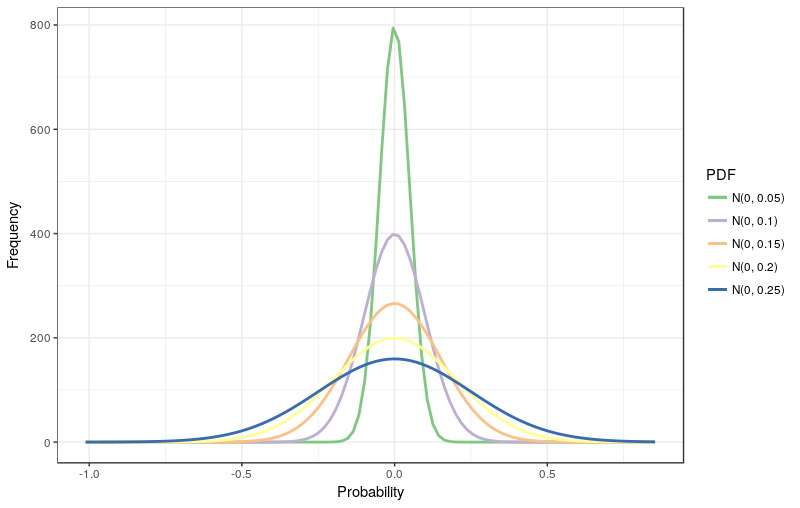
\includegraphics[width=0.8\textwidth]{img/gld_clustering/extra_images/5_gaussian.png}
    \caption{Gaussian (Normal) distributions used to generate the synthetic dataset.}
    \label{fig:5_gaussian}
\end{figure}

\begin{figure}[H]
    \centering
    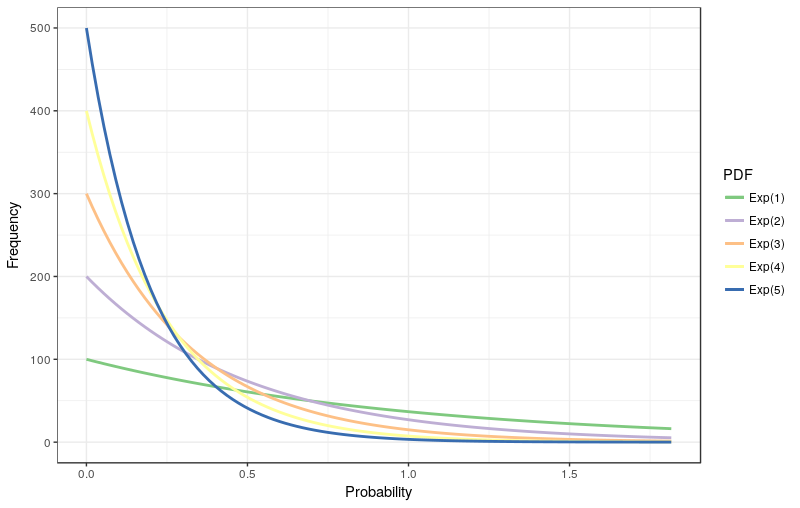
\includegraphics[width=0.8\textwidth]{img/gld_clustering/extra_images/5_exp.png}
    \caption{Exponential distributions used to generate the synthetic dataset.}
    \label{fig:5_exp}
\end{figure}

\begin{figure}[H]
    \centering
    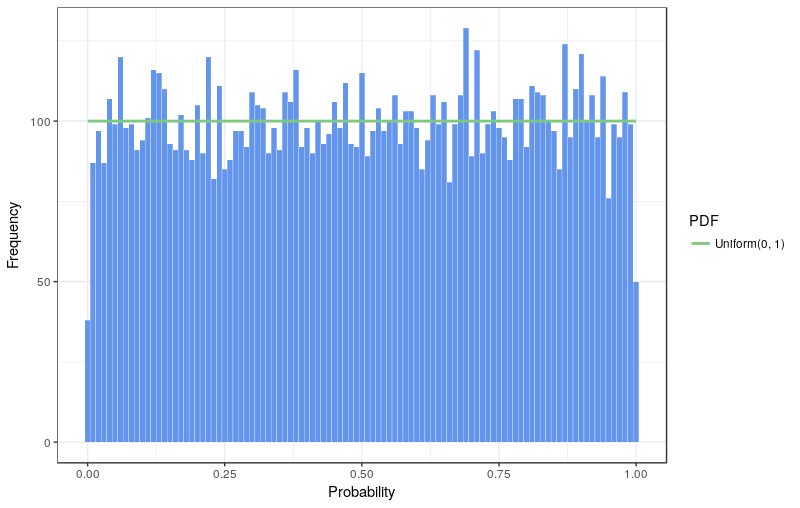
\includegraphics[width=0.8\textwidth]{img/gld_clustering/extra_images/uniform.png}
    \caption{Uniform distribution used to generate the synthetic dataset.}
    \label{fig:uniform}
\end{figure}

This dataset could be represented as a multidimensional array where for each position $x_{i}$, we have 1000 values $v_{j}$, equation \ref{eq:multi_array_datasetI}. In this case $i$ and $j$ vary from 1 to 1000 casually.

\begin{equation}\label{eq:multi_array_datasetI}
S(x_{i}, <v_{j}>) \quad i,j=1, 2.....1000
\end{equation}

The fitting algorithm proposed in subsection \ref{sub:fitting_gld} is applied over \ref{eq:multi_array_datasetI}. The good-of-fit test return that all the \textit{GLDs} are good fit for its corresponding distribution. As a result the dataset \ref{eq:multi_array3} is genarated. 

\begin{equation}\label{eq:multi_array3}
S(x_{i}, <\lambda_{1},\lambda_{2},\lambda_{3},\lambda_{4}>) \quad i=1.....1000
\end{equation}

\subsection{Clustering using $\lambda_{2}$, $\lambda_{3}$ and $\lambda_{4}$}\label{syntheticI_l234}

As we mention above, our idea is to test what happen if we use a simple k-means with euclidean distance over the $\lambda_{2}$, $\lambda_{3}$ and $\lambda_{4}$ values of the \textit{GLDs}. Similar to the paper \cite{Jiang2011}, as we use 11 \textit{PDFs} to generate the synthetic dataset I, we expect that the k-mean algorithm will return 11 clusters as well (one for each distribution). Then 11 is the number we use with the k-means algorithm.

In figure \ref{fig:dataset1_l2l3l4} and table \ref{tab:dataset1_l2l3l4} the distribution of the clusters returned by the k-means is shown.

\begin{figure}[H]
    \centering
    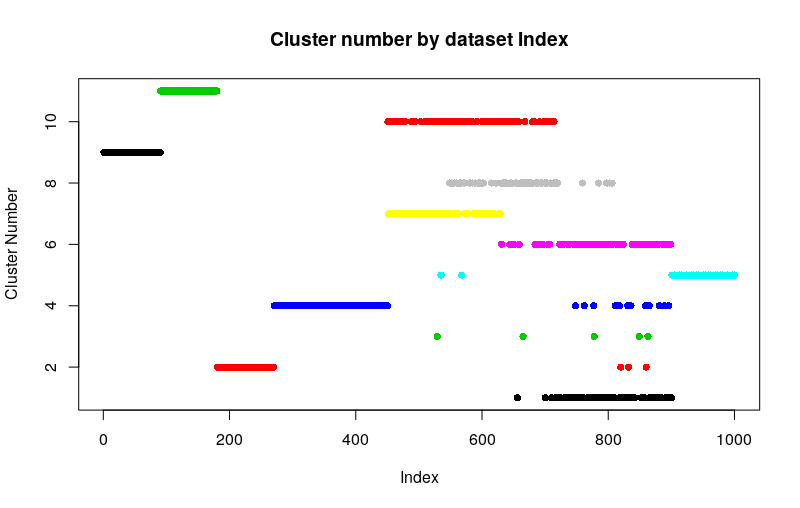
\includegraphics[width=0.8\textwidth]{img/gld_clustering/Dataset1/l2_l3_l4/intento_3/normal_exponential_uniform3.png}
    \caption{Distribution of the clusters using k-means over the $\lambda_{2}$, $\lambda_{3}$ and $\lambda_{4}$ values of the \textit{GLDs}.}
    \label{fig:dataset1_l2l3l4}
\end{figure}

\begin{table}[]
\centering
\caption{Distribution of the clusters using k-means over the $\lambda_{2}$, $\lambda_{3}$ and $\lambda_{4}$ values of the \textit{GLDs}.}
\label{tab:dataset1_l2l3l4}
\begin{tabular}{|c|c|c|}
\hline
Cluster & Type of Distribution & No. of Elements \\ \hline
1       & Exponential          & 82              \\ \hline
2       & Normal          & 93              \\ \hline
3       & Exponential          & 5             \\ \hline
4       & Normal               & 198              \\ \hline
5       & Uniform               & 102              \\ \hline
6       & Exponential               & 83             \\ \hline
7       & Exponential              & 91             \\ \hline
8       & Exponential          & 82              \\ \hline
9       & Normal          & 90               \\ \hline
10      & Exponential               & 84              \\ \hline
11      & Normal          & 90              \\ \hline
\end{tabular}
\end{table}

Remembered, the first 450 elements are normal distributions, the next 450 are exponential and the last 100 are uniform. Looking to those regions in general, the first observation is that we have 23 false positives, three in cluster 2, 18 in cluster 4 and two in cluster 5. The second observation is that, the normal distributions were grouped in 4 clusters (2, 4, 9 and 11), cluster 2 group perfectly it 90 elements with 2 false positives, clusters 9 and 11 group exactly its 90 elements each. The cluster 4 group the last 180 elements of the Normal distribution, with 18 false positives

The Uniform distribution was grouped totally in cluster 5, with two false positives as was mention above. The last observation is that the algorithm can't separate the 5 Exponential distributions, but this is not a bad result as we will show soon. 

In figures between \ref{fig:dataset1_l2l3l4_cl1} and \ref{fig:dataset1_l2l3l4_cl11} we show the \textit{PDFs} of all the distributions that belongs to the same cluster. If we take a look at figures \ref{fig:dataset1_l2l3l4_cl1}, \ref{fig:dataset1_l2l3l4_cl2}, \ref{fig:dataset1_l2l3l4_cl3}, \ref{fig:dataset1_l2l3l4_cl9}, \ref{fig:dataset1_l2l3l4_cl10} and \ref{fig:dataset1_l2l3l4_cl11} we see that the exponential distribution was well grouped. Really the problem is that the rate value of $0.05*i$ used to generate the exponential distribution does not have such a big difference between one and another.  

\begin{figure}[H]
    \centering
    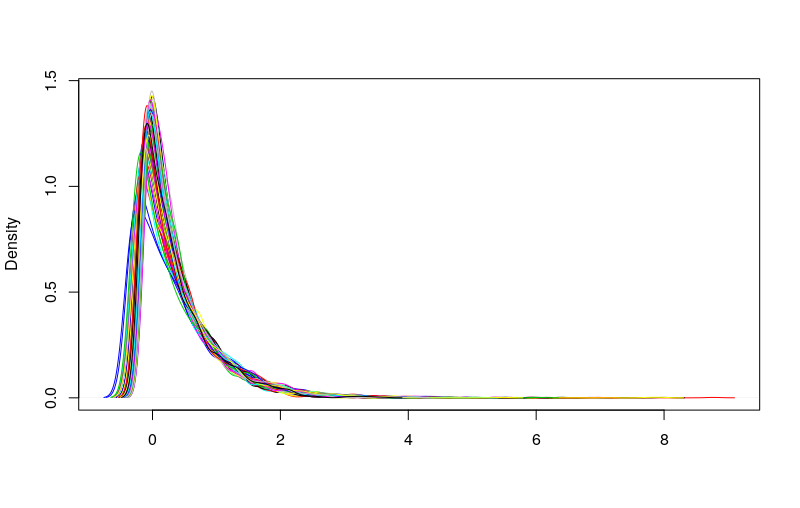
\includegraphics[width=0.8\textwidth]{img/gld_clustering/Dataset1/l2_l3_l4/intento_3/cluster1.png}
    \caption{Cluster 1 returned by the k-means over the $\lambda_{2}$, $\lambda_{3}$ and $\lambda_{4}$ values of the \textit{GLDs}, synthetic dataset I.}
    \label{fig:dataset1_l2l3l4_cl1}
\end{figure}

\begin{figure}[H]
    \centering
    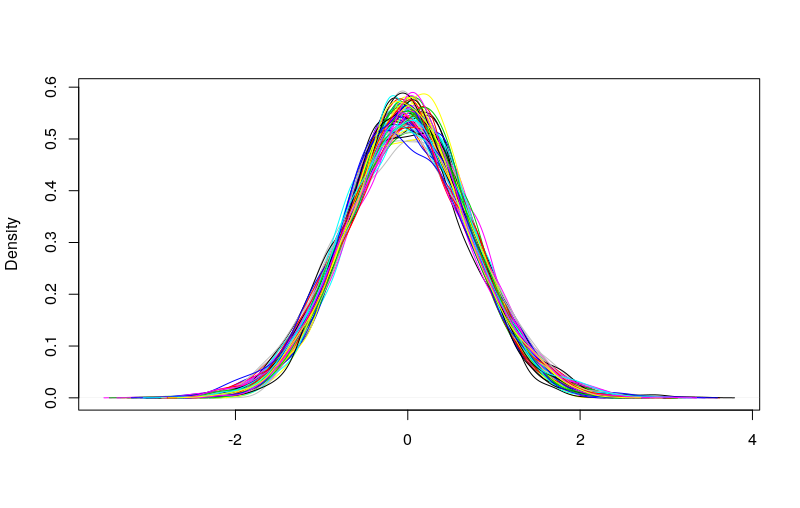
\includegraphics[width=0.8\textwidth]{img/gld_clustering/Dataset1/l2_l3_l4/cluster4.png}
    \caption{Cluster 2 returned by the k-means over the $\lambda_{2}$, $\lambda_{3}$ and $\lambda_{4}$ values of the \textit{GLDs}, synthetic dataset I.}
    \label{fig:dataset1_l2l3l4_cl2}
\end{figure}

\begin{figure}[H]
    \centering
    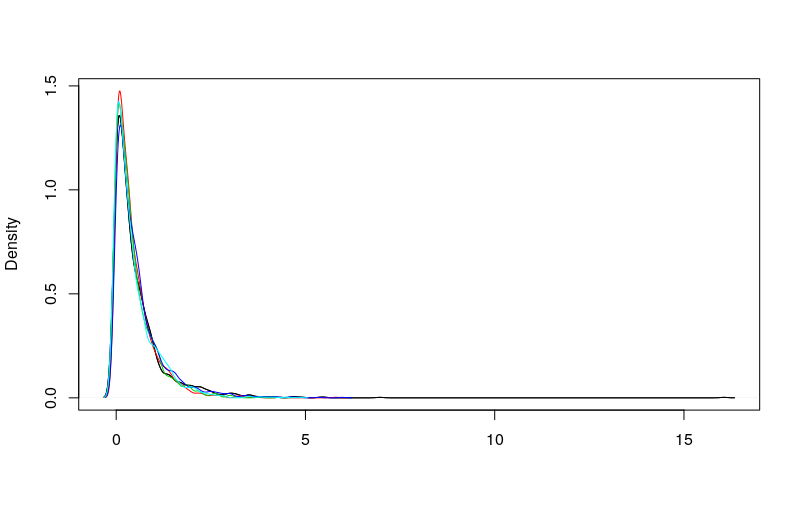
\includegraphics[width=0.8\textwidth]{img/gld_clustering/Dataset1/l2_l3_l4/intento_3/cluster3.png}
    \caption{Cluster 3 returned by the k-means over the $\lambda_{2}$, $\lambda_{3}$ and $\lambda_{4}$ values of the \textit{GLDs}, synthetic dataset I.}
    \label{fig:dataset1_l2l3l4_cl3}
\end{figure}

\begin{figure}[H]
    \centering
    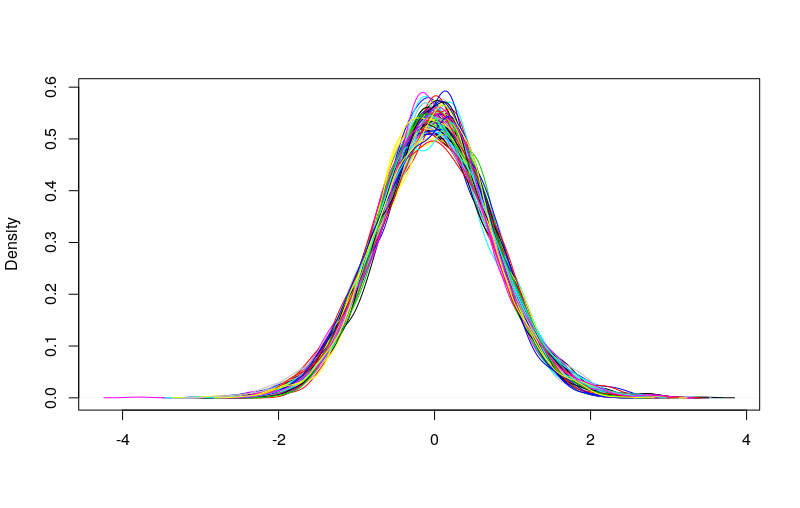
\includegraphics[width=0.8\textwidth]{img/gld_clustering/Dataset1/l2_l3_l4/cluster5.png}
    \caption{Cluster 4 returned by the k-means over the $\lambda_{2}$, $\lambda_{3}$ and $\lambda_{4}$ values of the \textit{GLDs}, synthetic dataset I.}
    \label{fig:dataset1_l2l3l4_cl4}
\end{figure}

\begin{figure}[H]
    \centering
    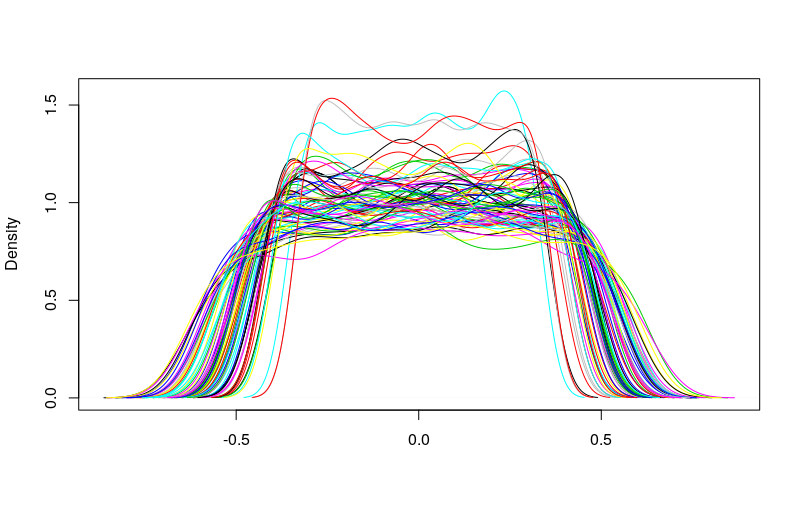
\includegraphics[width=0.8\textwidth]{img/gld_clustering/Dataset1/l2_l3_l4/cluster7.png}
    \caption{Cluster 5 returned by the k-means over the $\lambda_{2}$, $\lambda_{3}$ and $\lambda_{4}$ values of the \textit{GLDs}, synthetic dataset I.}
    \label{fig:dataset1_l2l3l4_cl5}
\end{figure}

\begin{figure}[H]
    \centering
    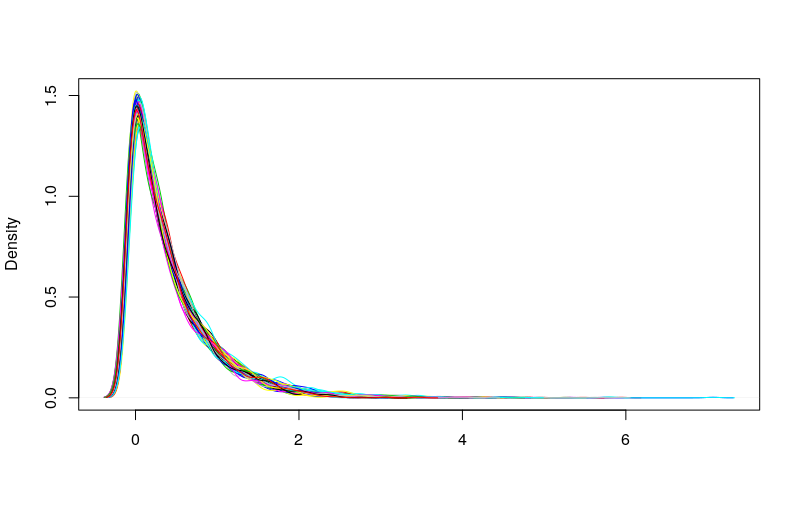
\includegraphics[width=0.8\textwidth]{img/gld_clustering/Dataset1/l2_l3_l4/intento_3/cluster6.png}
    \caption{Cluster 6 returned by the k-means over the $\lambda_{2}$, $\lambda_{3}$ and $\lambda_{4}$ values of the \textit{GLDs}, synthetic dataset I.}
    \label{fig:dataset1_l2l3l4_cl6}
\end{figure}

\begin{figure}[H]
    \centering
    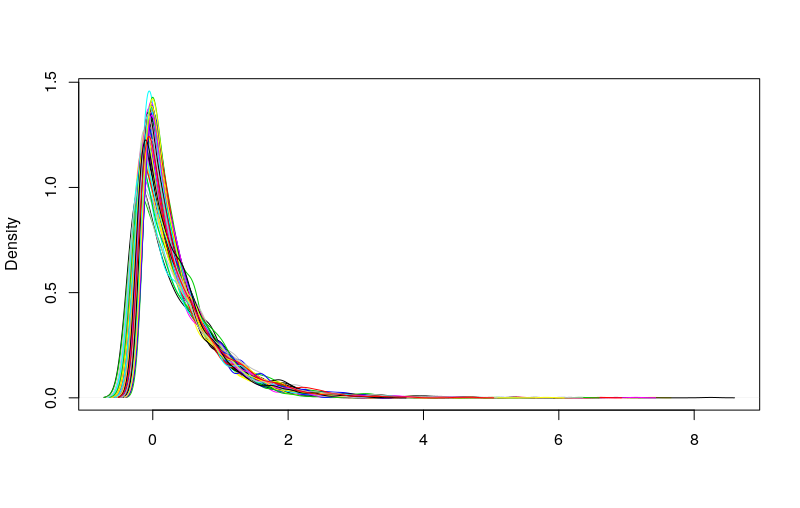
\includegraphics[width=0.8\textwidth]{img/gld_clustering/Dataset1/l2_l3_l4/intento_3/cluster7.png}
    \caption{Cluster 7 returned by the k-means over the $\lambda_{2}$, $\lambda_{3}$ and $\lambda_{4}$ values of the \textit{GLDs}, synthetic dataset I.}
    \label{fig:dataset1_l2l3l4_cl7}
\end{figure}

\begin{figure}[H]
    \centering
    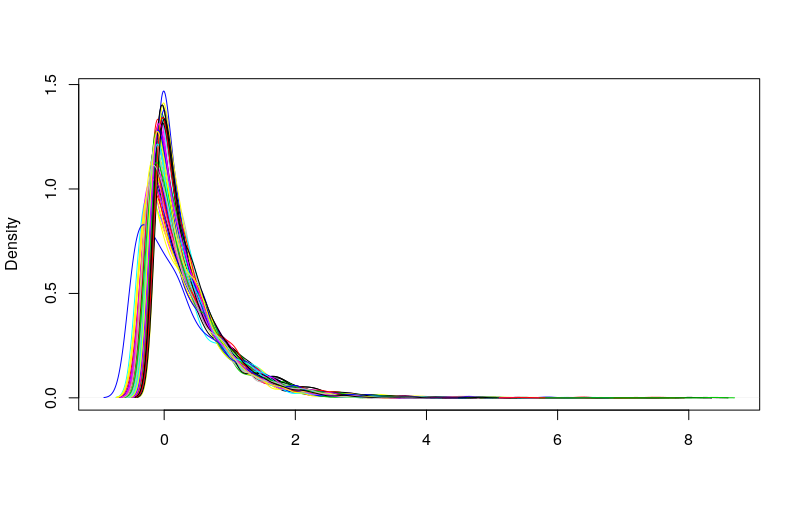
\includegraphics[width=0.8\textwidth]{img/gld_clustering/Dataset1/l2_l3_l4/intento_3/cluster8.png}
    \caption{Cluster 8 returned by the k-means over the $\lambda_{2}$, $\lambda_{3}$ and $\lambda_{4}$ values of the \textit{GLDs}, synthetic dataset I.}
    \label{fig:dataset1_l2l3l4_cl8}
\end{figure}

\begin{figure}[H]
    \centering
    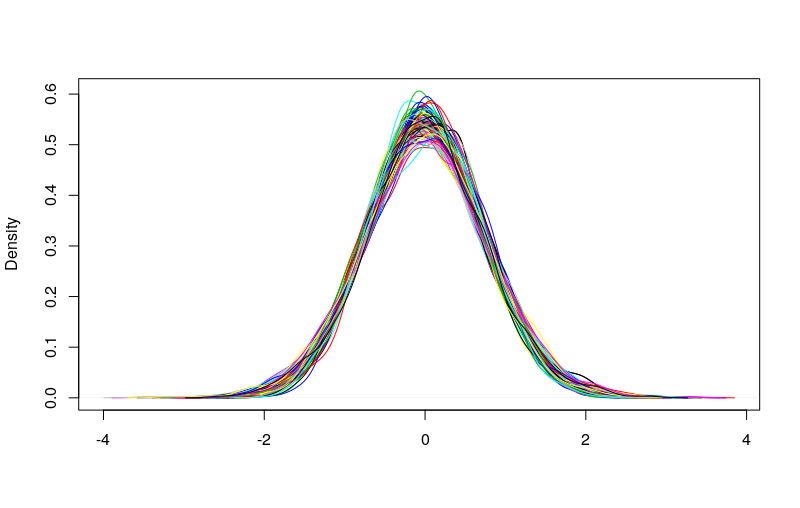
\includegraphics[width=0.8\textwidth]{img/gld_clustering/Dataset1/l2_l3_l4/intento_3/cluster9.png}
    \caption{Cluster 9 returned by the k-means over the $\lambda_{2}$, $\lambda_{3}$ and $\lambda_{4}$ values of the \textit{GLDs}, synthetic dataset I.}
    \label{fig:dataset1_l2l3l4_cl9}
\end{figure}

\begin{figure}[H]
    \centering
    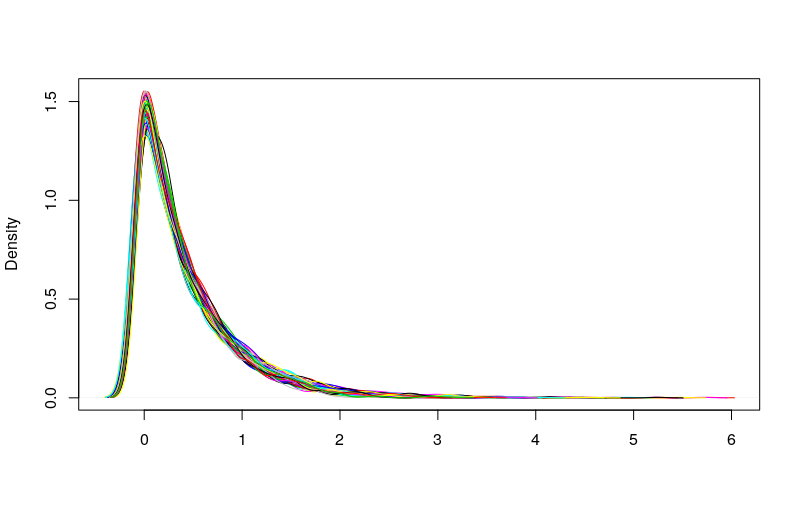
\includegraphics[width=0.8\textwidth]{img/gld_clustering/Dataset1/l2_l3_l4/intento_3/cluster10.png}
    \caption{Cluster 10 returned by the k-means over the $\lambda_{2}$, $\lambda_{3}$ and $\lambda_{4}$ values of the \textit{GLDs}, synthetic dataset I.}
    \label{fig:dataset1_l2l3l4_cl10}
\end{figure}

\begin{figure}[H]
    \centering
    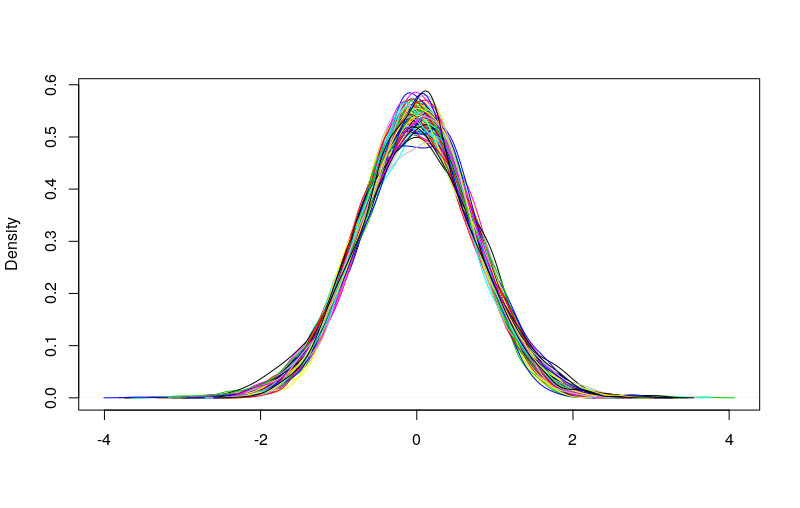
\includegraphics[width=0.8\textwidth]{img/gld_clustering/Dataset1/l2_l3_l4/intento_3/cluster11.png}
    \caption{Cluster 11 returned by the k-means over the $\lambda_{2}$, $\lambda_{3}$ and $\lambda_{4}$ values of the \textit{GLDs}, synthetic dataset I.}
    \label{fig:dataset1_l2l3l4_cl11}
\end{figure}

Another interesting result is show in figures \ref{fig:dataset1_l2l3l4_l3_l4} and \ref{fig:dataset1_l2l3l4_l3_l4_dividido}. As we can see, clusters 2, 4, 9 and 11 that represent the Normal distribution are all at the same region over the $\lambda_{3}$ and $\lambda_{4}$ space, near $\lambda_{3} = 0$ and $\lambda_{4} \in [0, 0.3]$. Similarly cluster 5, that represent the Uniform distribution is on the top left of the $\lambda_{3}$ and $\lambda_{4}$ space, $\lambda_{3} \in [0, 0.3]$ and $\lambda_{4} \in [0.7, 1.5]$. And finally the rest of the clusters that represent the Exponential distribution are distributed in the bottom of the $\lambda_{3}$ and $\lambda_{4}$ space, $\lambda_{3} \in [0.2, 7]$ and $\lambda_{4} \in [-0.1, 0.1]$. As we see in the rest of the thesis, this result is repeated in all the use cases.

\begin{figure}[H]
    \centering
    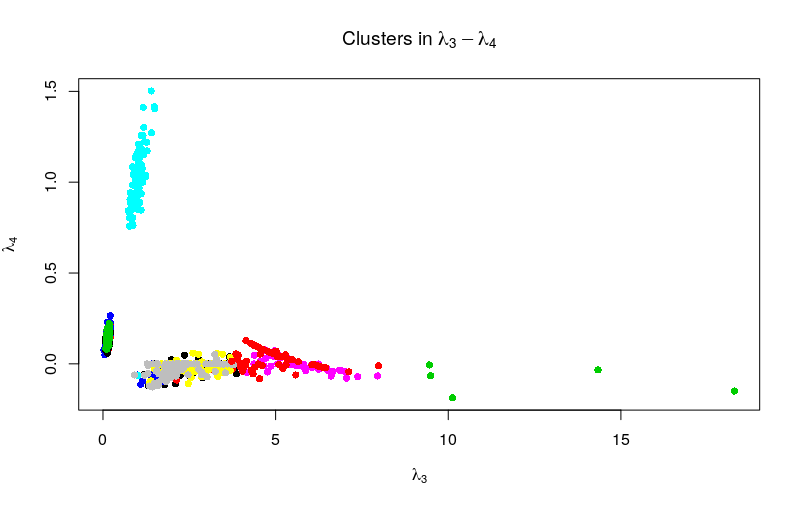
\includegraphics[width=0.8\textwidth]{img/gld_clustering/Dataset1/l2_l3_l4/intento_3/l3_l4.png}
    \caption{Distribution of the clusters over the $\lambda_{3}$ and $\lambda_{4}$ space.}
    \label{fig:dataset1_l2l3l4_l3_l4}
\end{figure}

\begin{figure}[H]
    \centering
    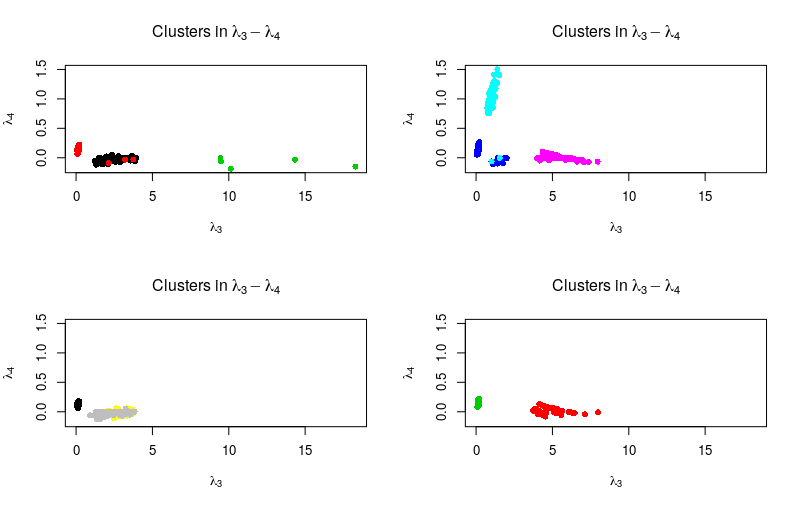
\includegraphics[width=0.8\textwidth]{img/gld_clustering/Dataset1/l2_l3_l4/intento_3/l3_l4_dividido.png}
    \caption{Distribution of the clusters over the $\lambda_{3}$ and $\lambda_{4}$ space. In the top left corner: clusters 1, 2 and 3. Top right corner: clusters 4, 5 and 6. Bottom left: clusters 7, 8 and 9. Bottom right: clusters 10 and 11.}
    \label{fig:dataset1_l2l3l4_l3_l4_dividido}
\end{figure}

\subsection{Clustering using $\lambda_{3}$ and $\lambda_{4}$}\label{syntheticI_l34}

In this section we proceed similar to section \ref{syntheticI_l234}, but the k-means algorithm run over $\lambda_{3}$ and $\lambda_{4}$. The distribution of the clusters is shown in figure \ref{fig:dataset1_l3l4} and table \ref{tab:dataset1_l3l4}.

\begin{figure}[H]
    \centering
    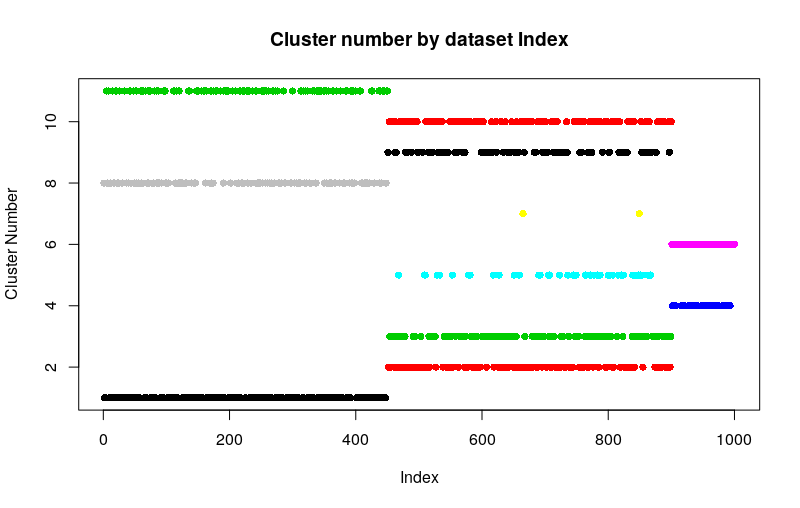
\includegraphics[width=0.8\textwidth]{img/gld_clustering/Dataset1/l3_l4/clusters_by_index.png}
    \caption{Distribution of the clusters using k-means over the $\lambda_{3}$ and $\lambda_{4}$ values of the \textit{GLDs}.}
    \label{fig:dataset1_l3l4}
\end{figure}

\begin{table}[]
\centering
\caption{Distribution of the clusters using k-means over the $\lambda_{3}$ and $\lambda_{4}$ values of the \textit{GLDs}.}
\label{tab:dataset1_l3l4}
\begin{tabular}{|c|c|c|}
\hline
Cluster & Type of Distribution & No. of Elements \\ \hline
1       & Normal          & 197              \\ \hline
2       & Exponential          & 118              \\ \hline
3       & Exponential          & 110             \\ \hline
4       & Uniform               & 35              \\ \hline
5       & Exponential               & 41              \\ \hline
6       & Uniform               & 65             \\ \hline
7       & Exponential              & 2             \\ \hline
8       & Normal          & 131              \\ \hline
9       & Exponential          & 74               \\ \hline
10      & Exponential               & 105              \\ \hline
11      & Normal          & 122              \\ \hline
\end{tabular}
\end{table}
 
 
As we don't use $\lambda_{2}$ here, is clear that the algorithm can't distinguish the distributions by its standard deviation. But, as the shape of the \textit{GLD} is defined by $\lambda_{3}$ and $\lambda_{4}$, what we expect is that the algorithm can separate the objects by type of distribution. As we see in figure \ref{fig:dataset1_l3l4} this is exactly what we get, there is no any false positive in this case, the three regions (Normal, Exponential and Uniform) are identified by the k-means.

Clusters 1, 8 and 11 group all the Normal distributions, clusters 4 and 6 group the Uniform and the rest group the Exponential.

In the $\lambda_{3}$ and $\lambda_{4}$ space the behavior is very similar at the one we get in subsection \ref{syntheticI_l234}, figures \ref{fig:dataset1_l3l4_l3_l4} and \ref{fig:dataset1_l3l4_l3_l4_dividido}. Again the distributions are concentrated near the same $(\lambda_{3}, \lambda_{4})$ values.

\begin{figure}[H]
    \centering
    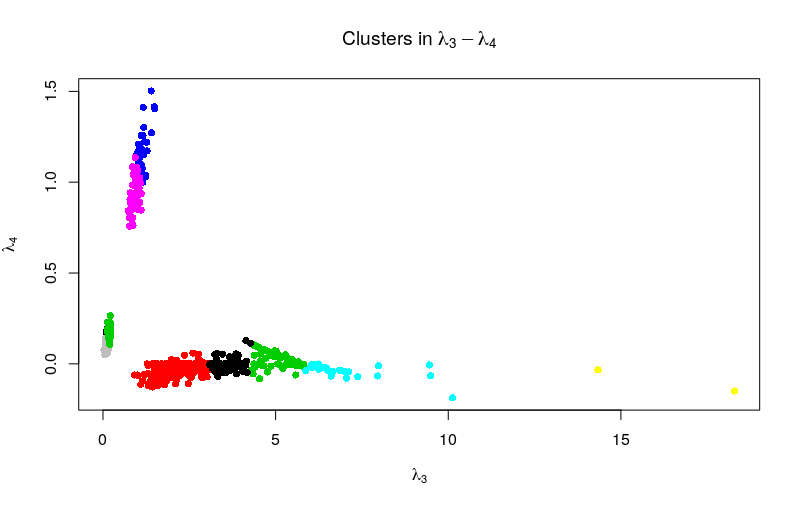
\includegraphics[width=0.8\textwidth]{img/gld_clustering/Dataset1/l3_l4/l3_l4.png}
    \caption{Distribution of the clusters over the $\lambda_{3}$ and $\lambda_{4}$ space.}
    \label{fig:dataset1_l3l4_l3_l4}
\end{figure}

\begin{figure}[H]
    \centering
    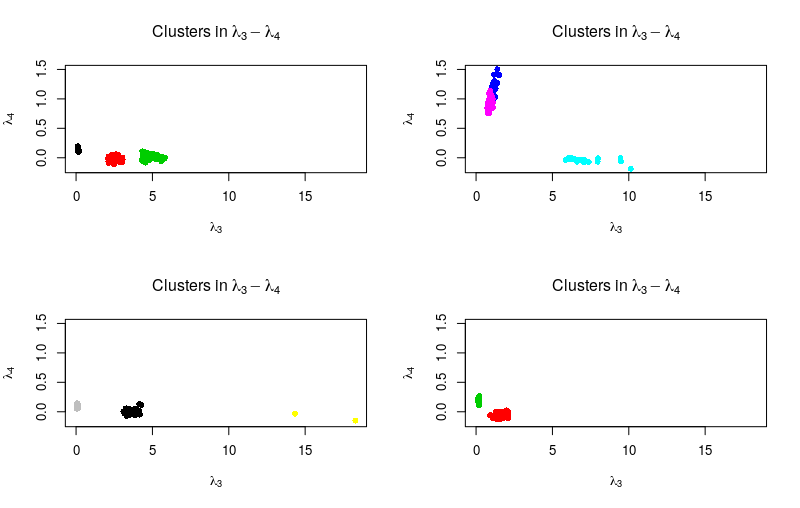
\includegraphics[width=0.8\textwidth]{img/gld_clustering/Dataset1/l3_l4/l3_l4_dividido.png}
    \caption{Distribution of the clusters over the $\lambda_{3}$ and $\lambda_{4}$ space. In the top left corner: clusters 1, 2 and 3. Top right corner: clusters 4, 5 and 6. Bottom left: clusters 7, 8 and 9. Bottom right: clusters 10 and 11.}
    \label{fig:dataset1_l3l4_l3_l4_dividido}
\end{figure}

%\subsection{Effectiveness of the Clustering}

\section{Synthetic Data II}\label{sec:synthetic_II}
The second synthetic dataset is similar to the first one, here we include 5 Gamma distributions, between the Exponential and the Uniform, figure \ref{fig:5_gamma}. The shape of the Gamma distribution is $i$, with $i=1, 2, 3, 4, 5$. This dataset have 1450 objects, where the first 450 were sampled from a Gaussian distributions, the next 450 from an Exponential, the next 450 are Gamma, and the last 100 from a Uniform distribution. As we use 16 different distributions, this is the number of clusters to be used with the k-means algorithm. 

\begin{figure}[H]
    \centering
    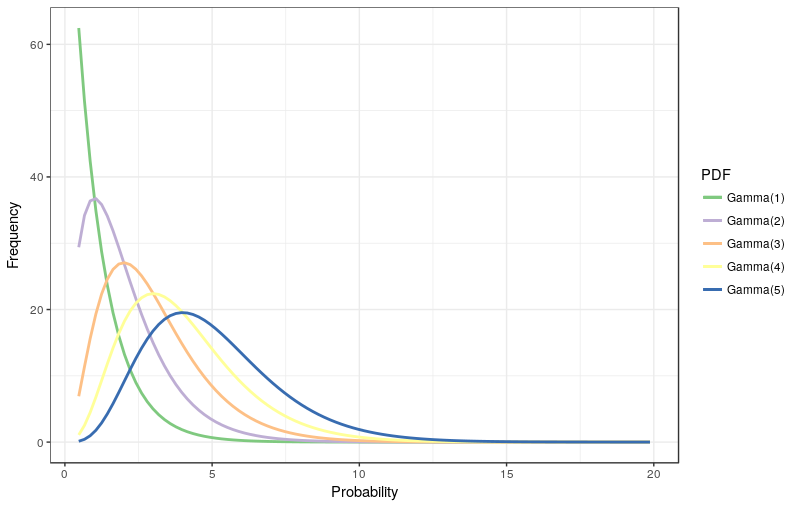
\includegraphics[width=0.8\textwidth]{img/gld_clustering/extra_images/5_gamma.png}
    \caption{Gamma distributions used to generate the synthetic dataset.}
    \label{fig:5_gamma}
\end{figure}

Similar to the dataset I, the fitting algorithm proposed in subsection \ref{sub:fitting_gld} is applied over dataset II. The good-of-fit test return that all the \textit{GLDs} are good fit for its corresponding distribution.

\subsection{Clustering using $\lambda_{2}$, $\lambda_{3}$ and $\lambda_{4}$}\label{syntheticII_l234}

The distribution of the clusters returned by the k-means algorithm is shown in figure \ref{fig:dataset2_l2l3l4} and table \ref{tab:dataset2_l2l3l4}.

\begin{figure}[H]
    \centering
    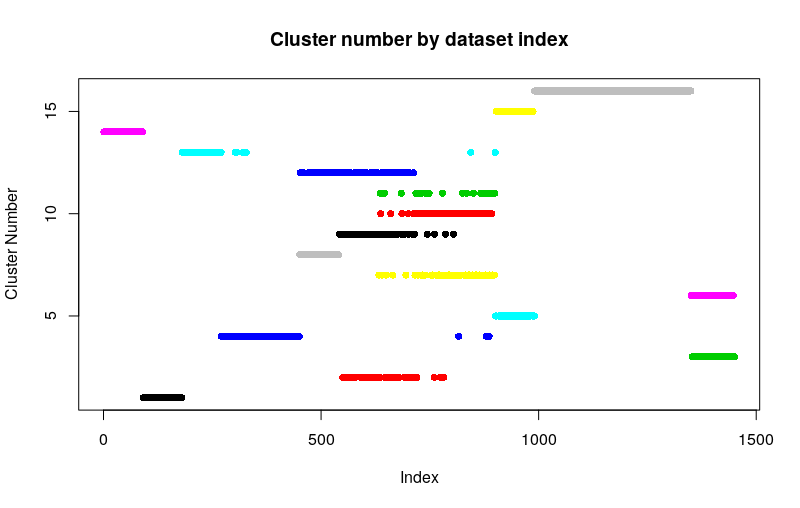
\includegraphics[width=0.8\textwidth]{img/gld_clustering/Dataset2/nuevo/clusters_by_index.png}
    \caption{Distribution of the clusters using k-means over the $\lambda_{2}$, $\lambda_{3}$ and $\lambda_{4}$ values of the \textit{GLDs}.}
    \label{fig:dataset2_l2l3l4}
\end{figure}

\begin{table}[]
\centering
\caption{Distribution of the clusters using k-means over the $\lambda_{2}$, $\lambda_{3}$ and $\lambda_{4}$ values of the \textit{GLDs}.}
\label{tab:dataset2_l2l3l4}
\begin{tabular}{|c|c|c|}
\hline
Cluster & Type of Distribution & No. of Elements \\ \hline
1       & Normal          & 90              \\ \hline
2       & Exponential          & 44              \\ \hline
3       & Uniform          & 45             \\ \hline
4       & Normal               & 179              \\ \hline
5       & Gamma               & 60             \\ \hline
6       & Uniform               & 55            \\ \hline
7       & Exponential              & 87            \\ \hline
8       & Exponential          & 58              \\ \hline
9       & Exponential          & 67               \\ \hline
10      & Exponential               & 74              \\ \hline
11      & Exponential          & 25              \\ \hline
12       & Exponential              & 90             \\ \hline
13       & Normal          & 96              \\ \hline
14       & Normal          & 90              \\ \hline
15      & Gamma               & 30              \\ \hline
16      & Gamma          & 360              \\ \hline
\end{tabular}
\end{table}

In general the results are very similar to the results of the section \ref{sec:synthetic_I}, but we get less false positives, 5 in total. 3 false positives in cluster 4 and 2 false positves in cluster 13. The normal distribution was groping again in for clusters: 1, 4, 13 and 14. The uniform distribution was grouping in clusters 3 and 6 without false positives. The gamma distribution introduced here was grouped in clusters 5, 15 and 16, without false positives. And finally the rest of the clusters are for the exponential distribution.

The projection of the clusters over the $\lambda_{3}$ and $\lambda_{4}$ space is show in figure \ref{fig:dataset2_l2l3l4_l3_l4}. The two clusters of the uniform distribution are located again in the top-left region of the figure. The normal distribution is located in the same place, near $\lambda_{3} = 0$ and $\lambda_{4} \in [0, 0.3]$. The exponential distribution is distributed in the bottom of the $\lambda_{3}$ and $\lambda_{4}$ space. The gamma distribution is overlapped together with the normal distribution.

\begin{figure}[H]
    \centering
    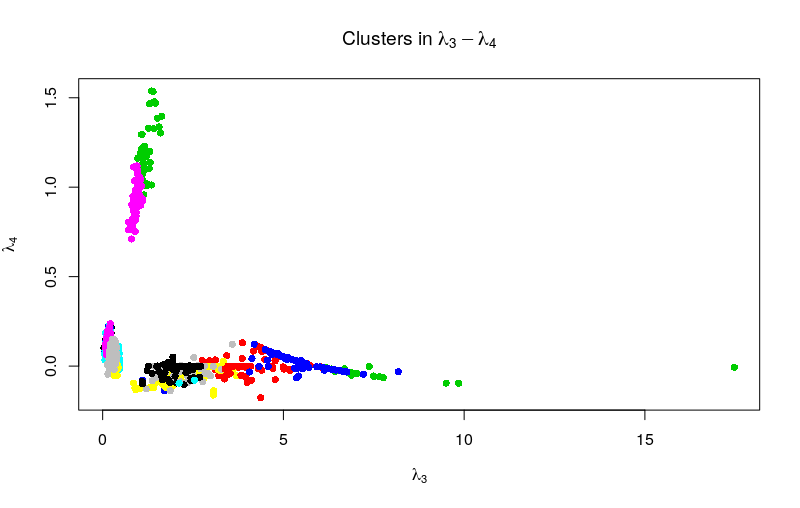
\includegraphics[width=0.8\textwidth]{img/gld_clustering/Dataset2/nuevo/l3_l4.png}
    \caption{Distribution of the clusters over the $\lambda_{3}$ and $\lambda_{4}$ space.}
    \label{fig:dataset2_l2l3l4_l3_l4}
\end{figure}

%\begin{figure}[H]
%    \centering
%    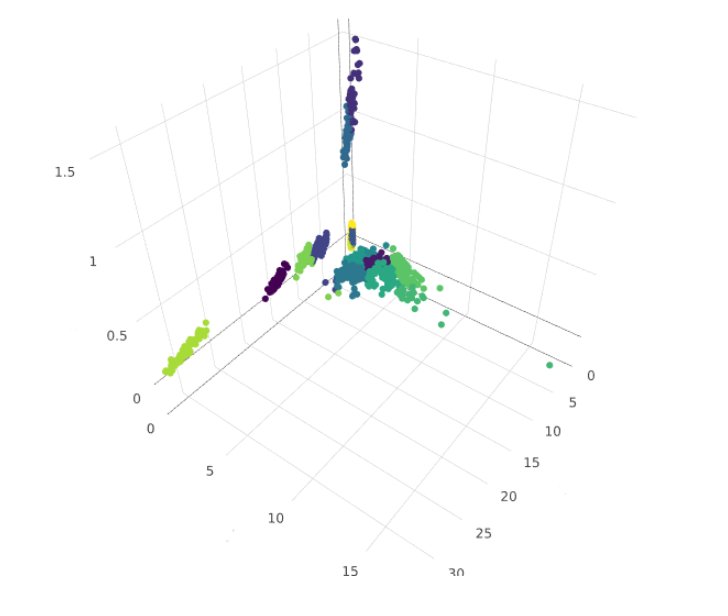
\includegraphics[width=0.8\textwidth]{img/gld_clustering/Dataset2/nuevo/l2_l3_l4_cortado.png}
%    \caption{Distribution of the clusters over the $\lambda_{2}$,  $\lambda_{3}$ and $\lambda_{4}$ space.}
%    \label{fig:dataset2_l2l3l4_l2_l3_l4}
%\end{figure}

\subsection{Clustering using $\lambda_{3}$ and $\lambda_{4}$}\label{syntheticI_l34}

The distribution of the clusters returned by the k-means when using the values of $\lambda_{3}$ and $\lambda_{4}$ to group the second synthetic dataset are shown in figure \ref{fig:dataset2_l3l4} and table \ref{tab:dataset2_l3l4}.
 
A few false positives are observed in clusters 5, 6 and 12, but nothing to worry about. Again the regions of the four distribution families are perfectly separated by the algorithm. 
 
\begin{table}[]
\centering
\caption{Distribution of the clusters using k-means over the $\lambda_{3}$ and $\lambda_{4}$ values of the \textit{GLDs}.}
\label{tab:dataset2_l3l4}
\begin{tabular}{|c|c|c|}
\hline
Cluster & Type of Distribution & No. of Elements \\ \hline
1       & Exponential          & 64              \\ \hline
2       & Exponential          & 126              \\ \hline
3       & Exponential          & 1             \\ \hline
4       & Exponential               & 57              \\ \hline
5       & Gamma               & 83             \\ \hline
6       & Normal               & 139            \\ \hline
7       & Uniform              & 67            \\ \hline
8       & Gamma          & 148              \\ \hline
9       & Gamma          & 108               \\ \hline
10      & Exponential               & 75              \\ \hline
11      & Exponential          & 80              \\ \hline
12       & Normal              & 112             \\ \hline
13       & Exponential          & 44              \\ \hline
14       & Normal          & 201              \\ \hline
15      & Gamma               & 112              \\ \hline
16      & Uniform          & 33              \\ \hline
\end{tabular}
\end{table}
 
 \begin{figure}[H]
    \centering
    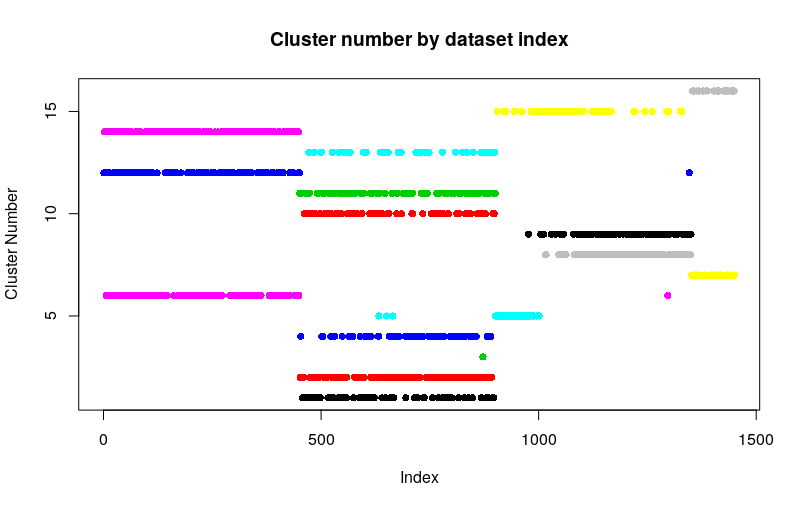
\includegraphics[width=0.8\textwidth]{img/gld_clustering/Dataset2/nuevo/l3_l4/clusters_by_index.png}
    \caption{Distribution of the clusters using k-means over the $\lambda_{2}$, $\lambda_{3}$ and $\lambda_{4}$ values of the \textit{GLDs}.}
    \label{fig:dataset2_l3l4}
\end{figure}

The projection of the clusters over the $\lambda_{3}$ and $\lambda_{4}$ space is show in figure \ref{fig:dataset2_l3l4_l3_l4}.

\begin{figure}[H]
    \centering
    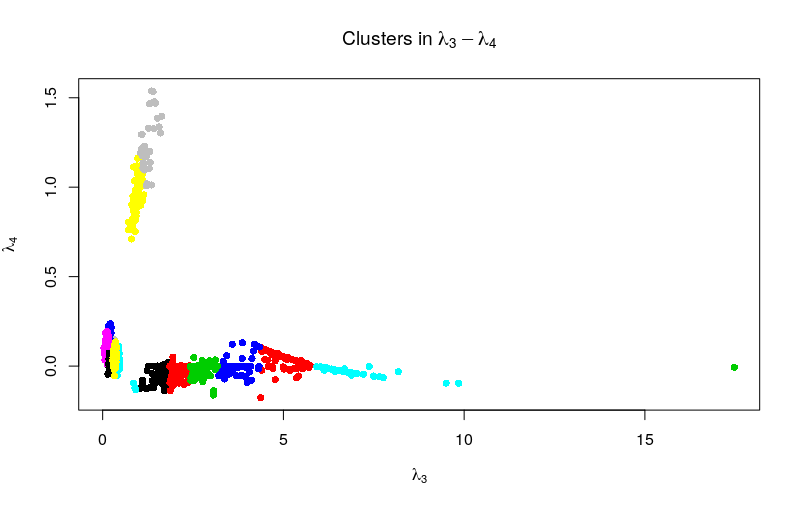
\includegraphics[width=0.8\textwidth]{img/gld_clustering/Dataset2/nuevo/l3_l4/l3_l4.png}
    \caption{Distribution of the clusters over the $\lambda_{3}$ and $\lambda_{4}$ space.}
    \label{fig:dataset2_l3l4_l3_l4}
\end{figure}

\section{Summary}\label{sec:clustering_summary}

In this Chapter, we explore clustering uncertain data based on the similarity between their distributions. The idea is to answer the \textbf{RQ.1} \textit{"how to group the output of the UQ process based on the similarity of the uncertainty?"}. The hypothesis enunciated at the beginning of the Chapter was tested against two synthetic datasets, and the results corroborate that we can group uncertain data based in the $\lambda_{i}$ values of the \textit{GLDs} that describe the data.

As a second result we test that, when using $\lambda_{2}$, $\lambda_{3}$ and $\lambda_{4}$ the separations of the different distributions of the dataset was almost perfect with a few false positives; and when using $\lambda_{3}$ and $\lambda_{4}$ all the elements of the same family are grouping together without consider the difference in the standard deviation. Both results are exactly what we expect.

Another important result of this Chapter, is that if we look at the clustering technique proposed here and compare it with the state-of-the-art, our approach is a competitive one. For example, in the approach proposed by \cite{Jiang} the computational cost of its algorithm depend of two factors, the fit of the distributions using Kernel Density Estimation (KDE) and the computation of the KL-divergence (the distance measure used in its approach). Both factors are computationally intensive. In our approach we substitute KDE by \textit{GLD} fit, that is most costly form the computational point of view; but at the same time we substitute the KL-divergence by simple distance comparisons in $\mathbf{R}$ and $\mathbf{R^2}$. On the other hand, some limitations of the KL-divergence approach as: (i) the \textit{PDF} of every uncertain object to be clustered need to be defined in the same domain and (ii) the needs to select an appropriate kernel to fit the data using KDE, are solved with the use of the \textit{GLD}.

All of this observation join with the rest of the advantage of the use of the \textit{GLD} to quantify the uncertainty, make our approach far superior to those reported in the literature.    